% \frame{\frametitle{The DRDoS attack}
% \begin{columns}
%   \begin{column}{0.6\textwidth}
%     \includegraphics[width=1\linewidth]{../image/drdos_1.pdf}
%   \end{column}
%   \begin{column}{0.4\textwidth}
%     \begin{itemize}
%     \item Attacker identifies a vulnerable service
%     \item Attacker sends requests to the service spoofing the IP to appear to be the victim
%     \end{itemize}
%   \end{column}
% \end{columns}
% }




\begin{frame}
  \frametitle{ Table of Contents}
  \begin{itemize}
  \item Introduction
  \item Automation and Labor
    \begin{itemize}
    \item Net Impact on Job Market
    \item Solutions to Impeding Problems
    \end{itemize}
  \item Ethical Questions in Automation
    \begin{itemize}
    \item Responsibility in Automated Systems
    \item Trust in Automated Systems
    \end{itemize}
  \item Questions
  \end{itemize}
\end{frame}


\begin{frame}
  \frametitle{ Ethical Automation: Introduction}
  \begin{itemize}
  \item A note on Labor
  \item A Brief Review of the Industrial Revolution(s)
  \item Big Question:
    \begin{itemize}
    \item We know automation destroys jobs.  How many does it make?
    \item What do we do when people lose their jobs?
    \end{itemize}
  \end{itemize}
\end{frame}


\begin{frame}
  \frametitle{ Ethical Automation: will automation create net job loss?}
  \begin{itemize} 
  \item
  \end{itemize}
\end{frame}


\begin{frame}
  \frametitle{ Ethical Automation: proposed solutions to job loss}
  \begin{itemize}
  \item
  \end{itemize}
\end{frame}

\begin{frame}
  \frametitle{ Ethical Automation: A brief aside}
  \begin{itemize}
  \item From Worker to Product
    \begin{itemize}
    \item We've talked about a worker being replaced by a machine
    \item How do we talk about those machines?
    \end{itemize}
  \item What is Responsibility?
  \item The Big Questions:
    \begin{itemize}
    \item When a machine fails, who is responsible?
    \item What kind of failure is acceptable?
    \end{itemize}
  \end{itemize}
\end{frame}


\begin{frame}
  \frametitle{ Ethical Automation: Responsibility in Automation}
  \Large{Responsiblity}
\end{frame}


\begin{frame}
  \frametitle{ Ethical Automation: Responsibility in Automation}
  {\Large Self-Driving Cars}
  \begin{itemize}
  \item The manufacturer is liable for failure, not the user
  \end{itemize}
\end{frame}


\begin{frame}
  \frametitle{ Ethical Automation: Responsibility in Automation}
  {\Large How Safe is Safe Enough?}\\
  424,331 autonomous miles. . . with a catch
  \begin{itemize}
  \item ``Safety Driver''
  \item Relinquished Control
  \item Emergency Intervention
  \end{itemize}
\end{frame}


\begin{frame}
  \frametitle{ Ethical Automation: Trust in Automation}
  \Large{Is it Moral to Trust the Morality of a Machine?}
\end{frame}


\begin{frame}
  \frametitle{ Ethical Automation: Trust in Automation}
  \begin{figure}[bht]
    \centering
    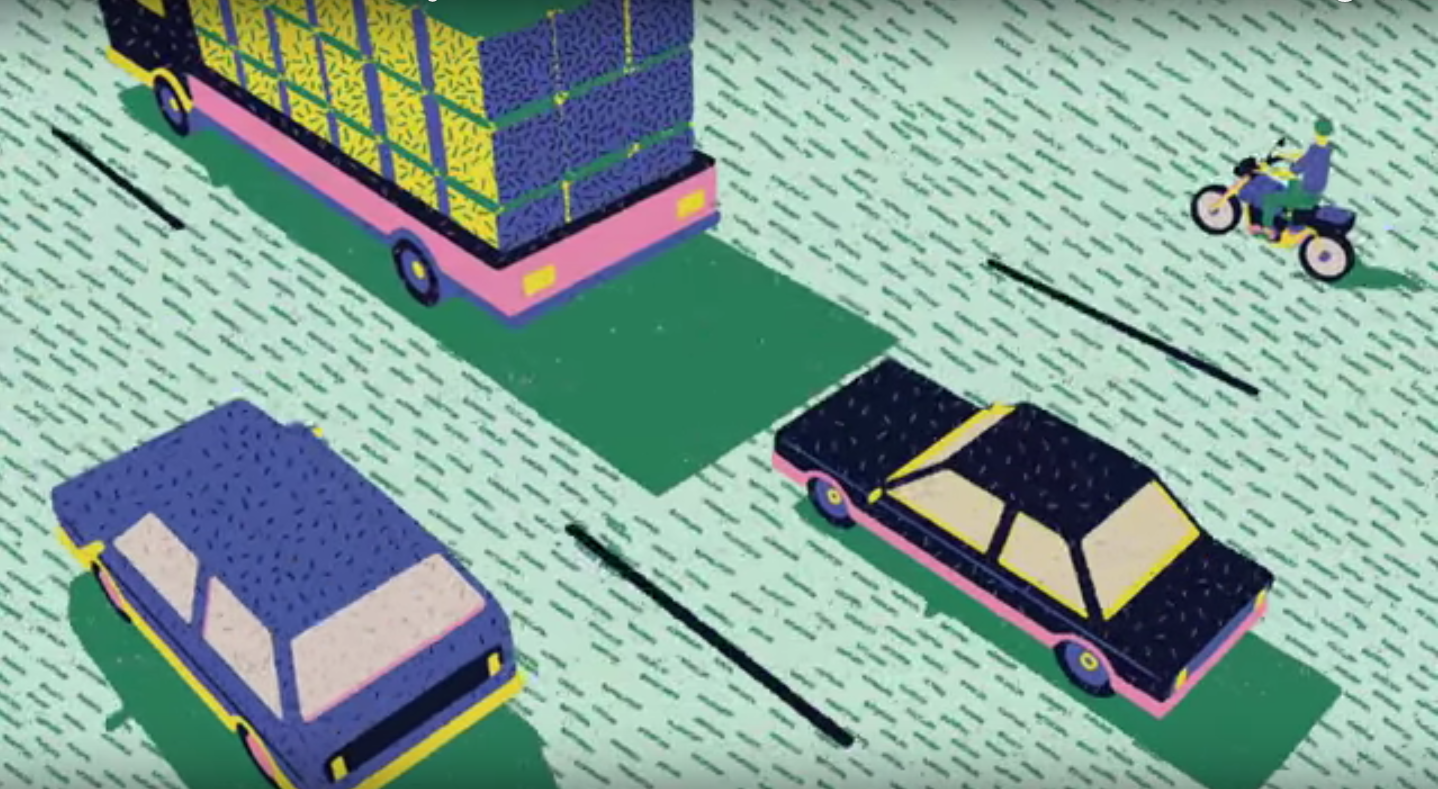
\includegraphics[width=4.1in]{diagrams/image00}
    \caption{An Ethical Scenario.}
    \label{fig:-deg}
  \end{figure}
\end{frame}


\begin{frame}
  \frametitle{ Ethical Automation: Trust in Automation}
  {\Large Reaction vs Decision}
  \begin{itemize}
  \item Humans react while machines decide
  \end{itemize}
\end{frame}


\begin{frame}
  \frametitle{ Ethical Automation: Trust in Automation}
  \begin{figure}[bht]
    \centering
    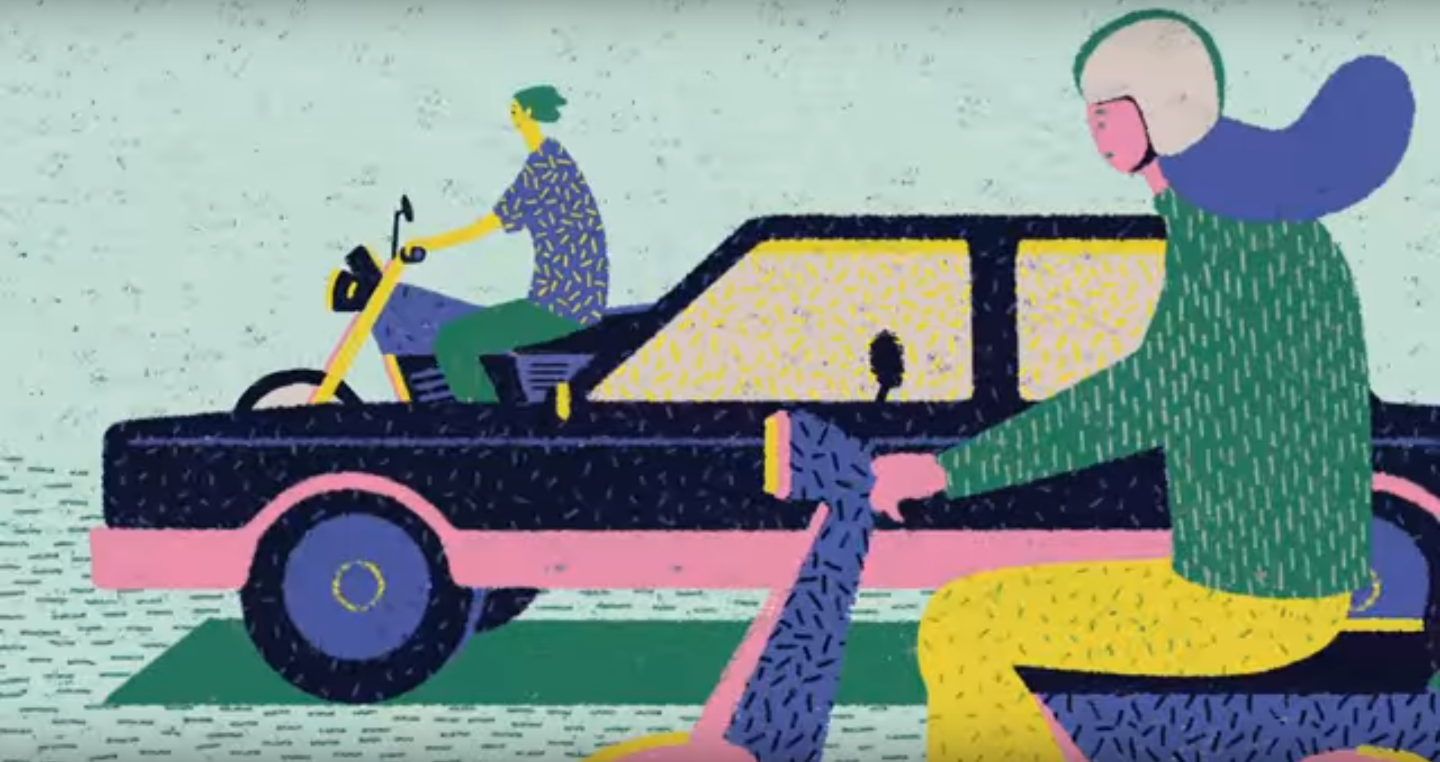
\includegraphics[width=4.1in]{diagrams/image01}
    \caption{}
    \label{fig:-deg}
  \end{figure}
\end{frame}


\begin{frame}
  \frametitle{ Ethical Automation: Trust in Automation}
  {\Large Conclusion}
  \begin{itemize}
  \item These moral dilemmas are too complicated and too controversial to decide.
  \end{itemize}
\end{frame}


\begin{frame}
  \frametitle{ Ethical Automation: Trust in Automation}
  \begin{itemize}
  \item
  \end{itemize}
\end{frame}
